\chapter{Funzioni di variabili casuali}
\label{sec:cambiamenti_variabile}

\`E giunto il momento di affrontare, almeno nel caso unidimensionale, un
problema che abbiamo toccato in superficie nella
sezione~\ref{sec:media_var_funzioni}---ovverosia quello del calcolo esplicito
della funzione di distribuzione di una \emph{funzione di variabile casuale}
$y = f(x)$, nota la funzione di distribuzione della variabile casuale $x$.

Può sembrare un argomento tecnico e, tutto sommato, di scarso interesse, ma
in questo capitolo vedremo che si tratta di un argomento fecondo di conseguenze,
ed alcuni dei risultati ci serviranno per inquadrare quantitativamente i
problemi di fit.


\section{Variabili discrete}

Cominciamo con il caso (relativamente semplice) di una variabile casuale
discreta. Uno potrebbe essere tentato di scrivere semplicemente
\begin{align}\label{eq:cambiamento_variabile_discr_biuniv}
  \prob{y = f(x_i)} = \prob{x = x_i}
\end{align}
ed in effetti questo è ciò che succede nel caso più elementare---quello
cioè in cui la funzione $f$ è biunivoca nell'intervallo di variabilità di
$x$ (vale a dire che per ogni valore $y_i$ di $y$ esiste uno ed un solo valore
$x_i$ di $x$ tale che $y_i$ è il trasformato di $x_i$ attraverso la nostra
funzione).

\begin{examplebox}
  \begin{example}
    Sia $x$ l'uscita di un dado equo a sei facce. La funzione di distribuzione
    della variabile casuale $y = x^2$ si può scrivere in forma tabellare come
    \begin{center}
      \begin{tabular}{lcccccc}
        \hline
        $x_i$ & $1$ & $4$ & $9$ & $16$ & $25$ & $36$\\
        \hline
        \hline
        $\prob{x_i}$ & \nicefrac{1}{6} & \nicefrac{1}{6} & \nicefrac{1}{6} &
        \nicefrac{1}{6} & \nicefrac{1}{6} & \nicefrac{1}{6}\\
        \hline
      \end{tabular}
    \end{center}
  \end{example}
\end{examplebox}

La situazione è leggermente più complicata se lasciamo cadere l'ipotesi di
biunivocità. \`E facile convincersi che in questo caso, preso un valore
(ammesso) della variabile $y$:
\begin{align}\label{eq:cambiamento_variabile_discr}
  \prob{y = f(x_i)} = \sum_{i=1}^{m} \prob{x = x_i}
\end{align}
dove la somma è estesa a tutti i valori (che qui supponiamo genericamente
essere $m$) di $x$ per cui $f(x_i) = \tilde y$. \`E più difficile a dirsi
che a farsi, e chiariamo il punto con l'esempio~\ref{exp:cambiamento_var_discr}.

\begin{examplebox}
  \begin{example}\label{exp:cambiamento_var_discr}
    Immaginiamo di avere un ipotetico dado simmetrico equo a sette facce---un
    oggetto cioè, la cui uscita $x$ sia descritta dalla funzione di
    distribuzione
    \begin{center}
      \begin{tabular}{lccccccc}
        \hline
        $x_i$ & $-3$ & $-2$ & $-1$ & $0$ & $1$ & $2$ & $3$\\
        \hline
        \hline
        $\prob{x_i}$ & \nicefrac{1}{7} & \nicefrac{1}{7} & \nicefrac{1}{7} &
        \nicefrac{1}{7} & \nicefrac{1}{7} & \nicefrac{1}{7} & \nicefrac{1}{7}\\
        \hline
      \end{tabular}
    \end{center}
    \`E chiaro che qui le cose non possono funzionare esattamente come prima.
    Per prima cosa la variabile casuale $y = x^2$ potrà assumere solo i
    4~valori $0,~1,~4,~9$ poiché, ad esempio, il valore $x_i = -2$ è
    trasformato in $y = 4$ dalla funzione $f(x)$ esattamente come $x_i = 2$.
    Allora avremo
    \begin{align*}
      \prob{y = 1} = \prob{x = -1} + \prob{x = 1} =
      \frac{1}{7} + \frac{1}{7} = \frac{2}{7},
    \end{align*}
    e la funzione di distribuzione di $y$ si scrive esplicitamente come:
    \begin{center}
      \begin{tabular}{lcccc}
        \hline
        $y_i$ & $0$ & $1$ & $4$ & $9$\\
        \hline
        \hline
        $\prob{y_i}$ & \nicefrac{1}{7} & \nicefrac{2}{7} & \nicefrac{2}{7} &
        \nicefrac{2}{7}\\
        \hline
      \end{tabular}
    \end{center}
  \end{example}
\end{examplebox}


\section{Variabili continue}

Il caso di una variabile casuale continua è quello di gran lunga più
interessante dal nostro punto di vista. Vedremo che le considerazioni che
abbiamo fatto a proposito delle variabili discrete nella sezione precedente
si applicano anche qui---e vedremo che, non a caso, calcolare la funzione
di distribuzione di una funzione di variabile casuale nel caso continuo
corrisponde essenzialmente a fare un cambiamento di variabile in un integrale.

Partiamo dunque, come prima, dal caso più semplice---quello in cui la funzione
$f(x)$ è biunivoca nell'intervallo di variabilità di $x$. (Per semplicità
assumeremo anche che $f(x)$ sia derivabile nell'intervallo di interesse.)
La biunivocità della corrispondenza tra le due variabili assicura che se
$x$ è compresa in un intervallo (infinitesimo) centrato su un generico valore
$x_0$:
\begin{align*}
  x \in \cinterval{x_0 - dx}{x_0 + dx}
\end{align*}
allora (e solo allora) $y$ è compresa in un intervallo (infinitesimo)
\begin{align*}
  y \in \cinterval{y_0 - dy}{y_0 + dy} \quad \text{con} \quad
  y_0 = f(x_0) \quad \text{e} \quad
  dy = \abs{\td{f}{x}{x_0}} dx.
\end{align*}
(Se siete incerti su questo punto, tornate a leggere la
sezione~\ref{sec:propagazione_errrore_max} ed osservate con attenzione la
figura~\ref{fig:linearizzazione_errore_max}. Non abbiamo fatto niente di nuovo.)
Se la nostra funzione $f$ è biunivoca, possiamo anche invertirla per ottenere
un'espressione per la vecchia variabile in funzione della nuova, sia
puntualmente che in termini di differenziali
\begin{align*}
  x = f^{-1}(y) \quad \text{e} \quad
  dx = \abs{\td{f^{-1}}{y}{y}} dy.
\end{align*}
Ma questo è tutto quello che ci serve. Se indichiamo con $p_x(x)$ la densità
di probabilità della nostra variabile originaria e con $p_y(y)$ la
densità di probabilità della variabile trasformata (che è esattamente
quello che cerchiamo) allora l'unica cosa che dobbiamo garantire è che
la probabilità associata in intervalli infinitesimi corrispondenti sia
preservata
\begin{align*}
  p_y(y) dy = p_x(x) dx =
  p_x\left(f^{-1}(y)\right)\abs{\td{f^{-1}}{y}{y}} dy,
\end{align*}
che deve valere per qualsiasi $x$. In definitiva, la nostra legge di
trasformazione si legge
\begin{align}
  p_y(y) = p_x\left(f^{-1}(y)\right)\abs{\td{f^{-1}}{y}{y}}.
\end{align}
La prescrizione per il cambio di variabile si può dunque esprimere a parole
mediante il seguente processo a tre passi:
\begin{enumerate}
\item invertire la $f(x)$ per ricavare un'espressione
  $x = f^{-1}(y)$ per $x$ in funzione di $y$;
\item derivare rispetto a $y$ l'espressione ottenuta al punto 1;
\item la funzione di distribuzione cercata è uguale al prodotto della
  funzione di distribuzione $p_x(x)$ di $x$, espressa in funzione della nuova
  variabile $y$, moltiplicata per la derivata calcolata al punto 2.
\end{enumerate}

Se adesso rilasciamo la richiesta che $f(x)$ sia biunivoca, il ragionamento
procede sostanzialmente invariato, con l'unica differenza che adesso
dobbiamo fare una somma sulla molteplicità delle radici dell'equazione
$x = f^{-1}(y)$
\begin{align}
  p_y(y) = \sum_{i = 1}^m p_x\left(f^{-1}_i(y)\right)\abs{\td{f^{-1}_i}{y}{y}}.
\end{align}


\section{Un esempio significativo: il quadrato di una variabile casuale}
\label{sec:pdf_quadrato}

Anziché procedere discutendo la materia in termini astratti, preferiamo
illustrare quanto imparato fino a questo momento con due esempi concreti che ci
saranno utili nel seguito: il calcolo della funzione di distribuzione
del quadrato di una variabile casuale $x$ con media $\mu = 0$ e varianza
$\sigma^2 = 1$ distribuita uniformemente o Gaussianamente.

(Notiamo, per inciso, che si tratta di una situazione in cui le relazioni
approssimate per la media e la varianza di una funzione di variabile casuale
che abbiamo ricavato nella sezione~\ref{sec:media_var_funzioni} falliscono
miseramente, poiché la derivata di $f(x) = x^2$ si annulla nel valor medio
della variabile casuale, ed il nostro sviluppo al prim'ordine è per
definizione privo di significato.)


\subsection{Il quadrato di una distribuzione uniforme}
\label{sec:pdf_quadrato_uniforme}

Consideriamo dunque una variabile casuale $x$ distribuita uniformemente tra
$-\sqrt{3}$ e $\sqrt{3}$---cioè con densità di probabilità
\begin{align*}
  p_x(x) = \left \{ \begin{array}{ll}
    \frac{\displaystyle 1}{\displaystyle 2\sqrt{3}} &
    -\sqrt{3} \leq x \leq \sqrt{3}\\
    0 & x < -\sqrt{3} ; ~ x > \sqrt{3}
  \end{array} \right.
\end{align*}
(se vi state chiedendo il motivo della scelta apparentemente curiosa
dell'intervallo, è semplice: questa è la distribuzione uniforme con media
$\mu = 0$ e deviazione standard $\sigma = 1$, come si può verificare
facilmente utilizzando i risultati che abbiamo ricavato nella
sezione~\ref{sec:distribuzione_uniforme}). Siamo interessati alla densità di
probabilità $p_y$ della variabile trasformata
\begin{align*}
  y = f(x) = x^2.
\end{align*}

Prima ancora di cominciare, notiamo che il valor medio di $y$ è banale da
calcolare grazie al fatto che la media di $x$ è nulla
\begin{align*}
  \expect{y} = \expect{x^2} = \sigma^2 + \mu^2 = \sigma^2 = 1.
\end{align*}
La nuova variabile $y$ è definita positiva, ed il supporto della densità di
probabilità che stiamo cercando sarà $\cinterval{0}{3}$. La distribuzione
di partenza è simmetrica rispetto ad $x = 0$, per cui per ogni $y > 0$ vi
sono esattamente due valori $x = \pm \sqrt{y}$ per cui $f(x) = y$---ed i valori
della funzione di distribuzione e del modulo della derivata di $f^{-1}$ sono
identici in questi due punti. Ne segue che la nostra somma si semplifica in
\begin{align*}
  p_y(y) = 2 p_x\left(f^{-1}(y)\right)\abs{\td{f^{-1}}{y}{y}},
\end{align*}
dove per $f^{-1}(y)$ intendiamo la radice positiva. I due ingredienti che ci
servono per calcolare $p_y$ sono dunque
\begin{align}
  x = f^{-1}(y) = \sqrt{y} \quad \text{e} \quad
  \td{f^{-1}}{y}{y} = \frac{1}{2\sqrt{y}} \quad \text{da cui} \quad
  p_y(y) = \frac{1}{2\sqrt{3y}}.
\end{align}

\pgffigone{quadrato_uniforme}{
  Grafico della funzione densità di probabilità del quadrato di una
  variabile casuale $x$ distribuita uniformemente tra $-\sqrt{3}$ e $\sqrt{3}$.
  (Per completezza la linea tratteggiata rappresenta la funzione di
  distribuzione della variabile di partenza.) \`E interessante notare come la
  densità di probabilità della variabile trasformata diverga in $x = 0$.
}

La densità di probabilità appena calcolata è mostrata in
figura~\ref{fig:quadrato_uniforme}. \`E facile verificare che la distribuzione,
così scritta, è correttamente normalizzata.
\begin{align*}
  \int_0^3 \frac{1}{2\sqrt{3y}} dy =
  \frac{1}{2\sqrt{3}} \int_0^3 \frac{1}{\sqrt{y}} \, dy =
  \eval{\left( \frac{y}{3} \right)^\frac{1}{2}}{0}{3} = 1.
\end{align*}
Per completezza calcoliamo esplicitamente media e varianza---anche se di fatto
la media la conosciamo già:
\begin{align}
  \expect{y} & = \int_0^3 yp_y(y) dy =
  \int_0^3 \frac{y}{2\sqrt{3y}} dy =
  \eval{\left(\frac{y}{3}\right)^{\frac{3}{2}}}{0}{3} = 1 \\
  \expect{y^2} & = \int_0^3 y^2p_y(y) dy =
  \int_0^3 \frac{y^2}{2\sqrt{3y}} dy =
  \eval{\frac{y^\frac{5}{2}}{5\sqrt{3}}}{0}{3} = \frac{9}{5}
  \quad \text{da cui} \quad \var{y} = \frac{9}{5} - 1 = \frac{4}{5}.
\end{align}


\subsection{Il quadrato di una Gaussiana}
\label{sec:pdf_quadrato_gaussiana}

Passiamo ora ad un caso più interessante, ovvero il calcolo della funzione
di distribuzione del quadrato di una variabile Gaussiana $z$ in forma standard.
Avremo modo di vedere nel capitolo~\ref{sec:metodi_di_fit} come la questione
è collegata ai metodi di \fit.

La quasi totalità delle cose che abbiamo detto nella sezione precedente
sono ancora valide. \`E ancora vero che il valore di aspettazione di $y$ è
$1$, ed è ancora vero che per ogni $y > 0$ vi sono esattamente due valori
$x = \pm \sqrt{y}$ tali che $f(x) = y$, per cui si ha di nuovo
\begin{align*}
  p_y(y) = 2 p_x\left(f^{-1}(y)\right)\abs{\td{f^{-1}}{y}{y}}.
\end{align*}
(Una differenza notevole, se vogliamo, è che adesso il supporto della
densità di probabilità di $p_y(y)$ è l'intera semiretta $y \geq 0$.)
In effetti abbiamo già tutti gli ingredienti che ci servono, e dobbiamo
semplicemente sostituire $y = z^2$ a $z$ nella densità di probabilità della
Gaussiana e moltiplicare per la derivata della funzione di trasformazione
inversa
\begin{align}\label{eq:pdf_quadrato_gauss}
  p_y(y) = \frac{2}{\sqrt{2\pi}}\, e^{-\frac{y}{2}} \, \frac{1}{2\sqrt{y}} =
  \frac{e^{-\frac{y}{2}}}{\sqrt{2\pi y}}.
\end{align}

\pgffigone{quadrato_gaussiana}{
  Grafico della funzione densità di probabilità del quadrato di una
  variabile casuale $z$ Gaussiana in forma standard. (Per completezza la linea
  tratteggiata rappresenta la funzione di distribuzione della variabile di
  partenza.) Notiamo che anche qui la densità di probabilità della
  variabile trasformata diverge in $x = 0$.
}

Questa volta non (ri-)dimostriamo esplicitamente che l'espressione ottenuta è
correttamente normalizzata e che la media della distribuzione è
$\expect{y} = 1$, ma il calcolo della varianza è istruttivo e ci servirà nel
seguito. Integrando per parti si ottiene
\begin{align*}
  \expect{y^2} = \int_0^\infty \frac{y^2 e^{-\frac{y}{2}}}{\sqrt{2\pi y}} dy =
  \frac{1}{\sqrt{2\pi}} \int_0^\infty y^\frac{3}{2}\, e^{-\frac{y}{2}} dy =
  -\eval{\frac{2}{\sqrt{2\pi}} y^\frac{3}{2}\, e^{-\frac{y}{2}}}{0}{\infty} +
  \frac{3}{\sqrt{2\pi}} \int_0^\infty y^\frac{1}{2}\, e^{-\frac{y}{2}} dy.
\end{align*}
Ora, il primo termine si annulla, mentre nel secondo riconosciamo essenzialmente
la definizione del valor medio, che conosciamo già, per cui
\begin{align}
  \expect{y^2} = 3 \expect{y} = 3 \quad \text{e} \quad \var{y} = 3 - 1 = 2.
\end{align}
Il quadrato di una variabile casuale Gaussiana in forma standard ha media $1$
e varianza $2$---teniamolo a mente perché ci sarà utile tra un attimo.


\section{La distribuzione del \texorpdfstring{$\chisq$}{chi2}}
\label{sec:pdf_chi2}

Il risultato ottenuto nella sezione~\ref{sec:pdf_quadrato_gaussiana} ci offre
lo spunto per introdurre una distribuzione che, pur non essendo strettamente
legata al tema principale di questo capitolo, ci sarà utile nel seguito.
Consideriamo la somma $x$ di $n$ variabili Gaussiane standard indipendenti
\emph{al quadrato}---che si indica solitamente, per ragioni che vedremo meglio
in seguito, con il nome di $\chisq$ a $n$ gradi di libertà
\begin{align}\label{eq:chi2}
  x = \sum_{i = 1}^n z_i^2.
\end{align}
Come si scrive la funzione di distribuzione di $x$? (Il problema non è proprio
banale, ed abbiamo detto che la pertinenza con il filo conduttore di questo
capitolo è limitata perché non si tratta di una funzione di una singola
variabile casuale, ma della somma di variabili casuali diverse ed indipendenti.)

Prima ancora di esaminare il problema in dettaglio, grazie al fatto che
sappiamo tutto sulla funzione di distribuzione di ciascuna delle $z_i^2$,
possiamo dire un certo numero di cose su $x$. In particolare nella
sezione~\ref{sec:media_varianza_somma} abbiamo ricavato le regole di somma
delle medie e delle varianze per variabili casuali indipendenti, che ci
permettono di scrivere banalmente
\begin{align}
  \label{eq:media_chi2}
  \expect{x} & = \sum_{i = 1}^n \expect{z_i^2} = \sum_{i = 1}^n 1 = n\\
  \label{eq:varianza_chi2}
  \var{x} & = \sum_{i = 1}^n \var{z_i^2} = \sum_{i = 1}^n 2 = 2n.
\end{align}
Inoltre sappiamo che, per il teorema centrale del limite, la funzione di
distribuzione di $x$ tende ad una gaussiana---con media e varianza date
dalle~\eqref{eq:media_chi2} e~\eqref{eq:varianza_chi2}---per
$n \rightarrow \infty$.

\pgffigsix[p]{pdf_chi2_1}{pdf_chi2_2}{pdf_chi2_3}{pdf_chi2_5}{pdf_chi2_10}{pdf_chi2_50}{
  Esempi di distribuzione del $\chisq$. Al variare del numero di gradi di
  libertà $n$ la~\eqref{eq:pdf_chi2} genera una varietà notevole di forme
  differenti. Per $n = 1$ essa coincide con la densità di probabilità di
  una variabile Gaussiana in forma standard al
  quadrato~\eqref{eq:pdf_quadrato_gauss} e per $n = 2$ con una distribuzione
  esponenziale~\eqref{eq:exponential_pdf} con media $\mu = 2$. Quando $n$ è
  molto grande la distribuzione del $\chisq$ tende ad una Gaussiana per il
  teorema centrale del limite.
}


Per completezza forniamo, senza dimostrazione, la soluzione completa del
problema, nella forma della distribuzione del $\chisq$
\begin{align}\label{eq:pdf_chi2}
  \chisquarepdf[n]{x} =
  \frac{1}{2^\frac{n}{2}\Gamma(\nicefrac{n}{2})}\, x^{\frac{n}{2} - 1} e^{-\frac{x}{2}}.
\end{align}
\`E facile verificare per sostituzione diretta che la funzione di distribuzione
di una variabile Gaussiana in forma standard al quadrato che abbiamo ricavato
nella sezione~\ref{sec:pdf_quadrato_gaussiana} non è altro che un $\chisq$
ad $1$ grado di libertà. Per $2$ gradi di libertà, viceversa, la
distribuzione del $\chisq$ si riduce alla distribuzione
esponenziale~\eqref{eq:exponential_pdf} con media $\mu = 2$.
Vari esempi di distribuzione del $\chisq$, per valori diversi del numero di
gradi di libertà, sono mostrati in figura~\ref{fig:pdf_chi2_1_six}.
Anticipiamo che la funzione cumulativa per una variabile $\chisq$ è
tabulata in appendice~\ref{sec:tavola_chisq1}.


\section{Un caso peculiare: la distribuzione di Cauchy}

Consideriamo una variabile casuale continua $\phi$ distribuita uniformemente
nell'intervallo $\cinterval{-\nicefrac{\pi}{2}}{\nicefrac{\pi}{2}}$
\begin{align*}
  p_\phi(\phi) = \left \{ \begin{array}{ll}
    \displaystyle \frac{1}{\pi} &
    \displaystyle -\frac{\pi}{2} \leq \phi \leq \frac{\pi}{2}\\
    \displaystyle 0 & \displaystyle \phi < -\frac{\pi}{2};~\phi > \frac{\pi}{2}
  \end{array} \right.
\end{align*}
Siamo interessati a calcolare la forma esplicita della densità di
probabilità della variabile trasformata $x$ definita da
\begin{align}\label{eq:trasformazione_cauchy}
  x = f(\phi) = \gamma \tan \phi + x_0.
\end{align}

Prima di andare avanti con il calcolo, notiamo che questo problema ha
un'interessante interpretazione geometrica, mostrata in
figura~\ref{fig:geometria_cauchy}: se abbiamo una sorgente luminosa
posta a distanza $\gamma$ da uno schermo infinito (in corrispondenza di un
punto fissato $x_0$) che emette uniformemente in tutte le direzioni, allora
$x$ rappresenta la distribuzione dei punti di intersezione dei raggi con lo
schermo stesso.

\begin{figure}[htb!]
  \autohstack{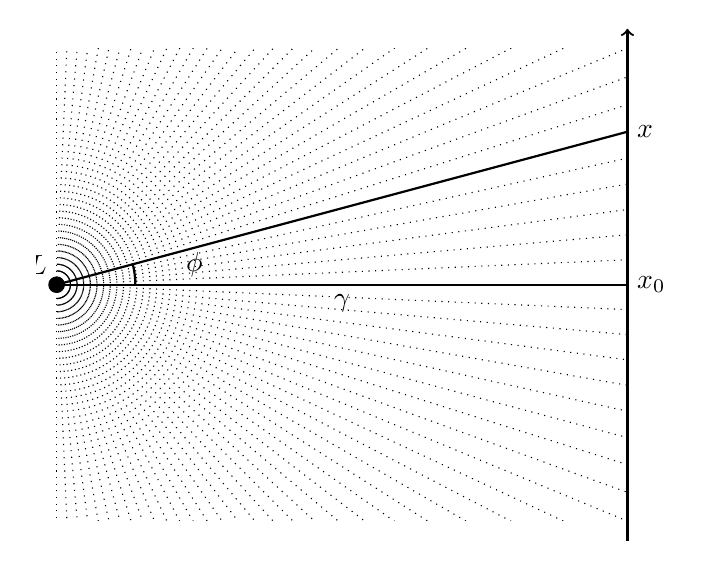
\begin{tikzpicture}
  \pgfmathsetmacro{\d}{0.25}
  \pgfmathsetmacro{\w}{7.5}
  \pgfmathsetmacro{\h}{3.}
  \pgfmathsetmacro{\p}{15.}
  \node at (0, \h + 0.1) {};
  \node at (0, -\h - 0.1) {};
  \fill (\d, 0) circle [radius=3pt];
  \draw[thick,-{>[scale=1.5]}] (\w, -\h - 0.25) -- (\w, \h + 0.25);
  \node[anchor=west] at (\w, 0) {$x_0$};
  \node[anchor=west] at (\w, {(\w - \d)*tan(\p)} ) {$x$};

  \clip (0, -\h) rectangle (\w + 0.5, \h);
  \foreach \phi in {-87.5, -85,...,87.5}
  \draw[style=dotted] (\d, 0) -- (\w, {(\w - \d)*tan(\phi)} );

  \draw[style=dotted] (\d, -2*\h) -- (\d, 2*\h);
  \draw[thick] (\d, 0) -- (\w, 0);
  \draw[thick] (\d, 0) -- (\w, {(\w - \d)*tan(\p)} );

  \node[anchor=north] at ({0.5*(\d + \w)}, 0) {$\gamma$};
  \draw[thick] (\d + 1, 0) arc (0:\p:1.05cm);
  \node at (1.75 + \d,0.25) {$\phi$};
  \node[anchor=south east] at (\d, 0) {$L$};
\end{tikzpicture}
}{
    \caption{Interpretazione geometrica della
      trasformazione~\eqref{eq:trasformazione_cauchy}. Se la sorgente luminosa
      $L$ è posta a distanza $\gamma$ dallo schermo in corrispondenza del
      punto $x_0$, $x$ rappresenta l'intersezione con lo schermo stesso del
      generico raggio di luce emesso ad un angolo $\phi$.}
    \label{fig:geometria_cauchy}
  }
\end{figure}

Cominciamo, al solito, scrivendo la trasformazione inversa e derivando la
relazione ottenuta rispetto alla variabile trasformata $x$:
\begin{align*}
  \phi = f^{-1}(x) = \arctan\left(\frac{x - x_0}{\gamma}\right),
  \quad \text{da cui} \quad
  \td{f^{-1}}{x}{x} = \frac{\gamma}{(x - x_0)^2 + \gamma^2}.
\end{align*}
A questo punto è banale trovare la densità di probabilità di $x$---si
tratta essenzialmente di moltiplicare per $\nicefrac{1}{\pi}$. La funzione di
distribuzione di $x$ di dice distribuzione di Cauchy (o, a seconda del contesto,
distribuzione di Lorentz, Lorentziana o distribuzione di Breit-Wigner) e si
scrive come
\begin{align}\label{eq:pdf_cauchy}
  \cauchypdf[x_0, \gamma]{x} =
  \frac{1}{\pi} \left[\frac{\gamma}{(x - x_0)^2 + \gamma^2} \right].
\end{align}
Notiamo esplicitamente che la distribuzione di Cauchy dipende da due parametri:
il \emph{parametro di posizione} $x_0$ ed il \emph{parametro di scala} $\gamma$.
Nel caso particolare $x_0 = 0$ e $\gamma = 1$, analogamente a quanto si fa per
la distribuzione di Gauss, si parla di distribuzione di Cauchy in forma
standard
\begin{align}\label{eq:pdf_cauchy_std}
  \cauchypdf[0, 1]{x} = \frac{1}{\pi(1 + x^2)}.
\end{align}
Le densità di probabilità corrispondenti sono confrontate in
figura~\ref{fig:pdf_cauchy}.

\pgffigone{pdf_cauchy}{
  Grafico della distribuzione di Cauchy in forma standard (cioè con
  parametro di posizione $x_0 = 0$ e parametro di scala $\gamma = 1$).
  Per confronto, la linea tratteggiata rappresenta una distribuzione di
  Gauss in forma standard. La differenza più rilevante tra le due sta
  nel fatto che le code della distribuzione di Cauchy sono significativamente
  più pronunciate.
}


\subsection{Alcune proprietà della distribuzione di Cauchy}

La distribuzione di Cauchy, così come è scritta nella~\eqref{eq:pdf_cauchy},
è correttamente normalizzata---e l'integrale è banale in quanto, avendo
ottenuto la densità di probabilità derivando la trasformazione inversa
(modulo una costante), abbiamo di fatto l'espressione esplicita per la
primitiva della densità di probabilità stessa
\begin{align*}
  \int_{-\infty}^\infty \cauchypdf[x_0, \gamma]{x} \diff =
  \int_{-\infty}^\infty \frac{1}{\pi}
  \left[\frac{\gamma}{(x - x_0)^2 + \gamma^2} \right] \diff =
  \frac{1}{\pi}
  \eval{\arctan\left(\frac{x - x_0}{\gamma}\right)}{-\infty}{\infty} \;\; =
  \frac{1}{\pi}\left(\frac{\pi}{2} + \frac{\pi}{2}\right) = 1.
\end{align*}
Per inciso, questo ci permette immediatamente di calcolare la funzione
cumulativa e la funzione di distribuzione inversa per la distribuzione in
questione---ovvero
\begin{align}
  F(x) = \frac{1}{2} + \frac{1}{\pi}\arctan\left(\frac{x - x_0}{\gamma}\right)
  \quad \text{e} \quad
  F^{-1}(q) = x_0 + \gamma\tan\left( \pi q - \frac{\pi}{2} \right).
\end{align}

Veniamo alle cose interessanti, e concentriamoci un attimo per semplicità
(ma senza perdere in generalità) sulla distribuzione in forma
standard~\eqref{eq:pdf_cauchy_std}. La nostra solita espressione per la media
\begin{align*}
  \expect{x} = \int_{-\infty}^\infty x\,\cauchypdf[0, 1]{x} \diff =
  \int_{-\infty}^\infty \frac{x}{\pi(1 + x^2)} \diff =
  \eval{\frac{1}{2\pi} \log(1 + x^2)}{-\infty}{\infty}
\end{align*}
porta in questo caso ad una forma indeterminata di tipo $\infty - \infty$%
\footnote{Non abbiamo gli strumenti per sviscerare l'argomento in tutti i suoi
  dettagli, ma vale la pena notare che la \emph{parte} principale dell'integrale
  che esprime la media
  \begin{align*}
    \lim_{c \rightarrow \infty} \int_{-c}^c x\,\cauchypdf[0, 1]{x}
  \end{align*}
  esiste ed è $0$, come uno si aspetterebbe intuitivamente sulla base che
  la distribuzione è pari. Purtroppo prescrizioni diverse sul limite
  portano a valori diversi dell'integrale per cui, come abbiamo detto,
  l'integrale stesso non è definito.
}
per cui siamo costretti ad ammettere che la distribuzione di Cauchy non ha
media definita. Questo è un problema---e non da poco---perché se la media
non è definita non possiamo definire i momenti centrali di ordine superiore,
primo tra tutti la varianza. Notiamo che se, in virtù del fatto che la
funzione di distribuzione è pari, volessimo ignorare che la media non esiste
e provassimo a calcolare una sorta di pseudo-varianza come momento centrale
di ordine due, non andremmo molto lontano, poiché
\begin{align*}
  \expect{x^2} = \int_{-\infty}^\infty x^2\,\cauchypdf[0, 1]{x} \diff =
  \int_{-\infty}^\infty \frac{x^2}{\pi(1 + x^2)} \diff \rightarrow \infty.
\end{align*}
(In questo caso, banalmente, l'integrando non tende a zero per
$x \rightarrow \pm \infty$.) Il fatto che questo integrale diverga, fisicamente,
è dovuto alle code della distribuzione, che sono molto più accentuate
rispetto al caso, e.g., della Gaussiana. Più in generale possiamo dire che
tutti i momenti algebrici di ordine dispari della distribuzione di Cauchy
sono indefiniti e tutti i momenti algebrici di ordine pari divergono; questo
vale in generale---non solo per la distribuzione in forma standard.

Notiamo anche, per completezza, che la mediana e la moda
della~\eqref{eq:pdf_cauchy_std} sono entrambi pari al parametro di posizione
$x_0$. La semilarghezza a metà altezza è data dalla soluzione (per la
quantità $x - x_0$) dell'equazione
\begin{align*}
  \frac{1}{\pi} \left[\frac{\gamma}{(x - x_0)^2 + \gamma^2} \right] =
  \frac{1}{2\pi\gamma} \quad \text{ovvero} \quad
  \hwhm = \gamma,
\end{align*}
cioè è pari al parametro di scala. In assenza di una media e di una
deviazione standard definite, la mediana e la semilarghezza a metà altezza
sono in questo caso le misure più utili di tendenza centrale e dispersione
intorno alla media.


\subsection{La distribuzione di Cauchy ed il teorema centrale del limite}

Se vi ricordate una delle ipotesi necessarie per la validità del teorema
centrale del limite è il fatto che le distribuzioni di partenza avessero
media e varianza finite. Ebbene, la figura~\ref{fig:tcl_cauchy_1_six}
illustra il fallimento spettacolare del teorema centrale del limite nel caso
della distribuzione di Cauchy (confrontatela con le
figure~\ref{fig:tcl_uniforme} e~\ref{fig:tcl_esponenziale}).
Osserviamo la situazione in dettaglio. Il primo problema è che, a parte la
scala sull'asse delle $x$, gli istogrammi in figura~\ref{fig:tcl_cauchy_1_six}
sono essenzialmente identici l'uno all'altro, indipendentemente dal valore di
$n$---cioè la loro forma non si avvicina, al crescere di $n$, ad una
distribuzione di Gauss. Il secondo problema è che la larghezza relativa degli
istogrammi cresce come $n$, anziché come $\sqrt{n}$, al crescere di $n$.
(Va da sé che nessuno dei due è un reale problema: la distribuzione di
Cauchy non ha media e varianza finite per cui semplicemente il teorema centrale
del limite non vale per la somma di distribuzioni di Cauchy.)

\pgffigsix{tcl_cauchy_1}{tcl_cauchy_2}{tcl_cauchy_3}{tcl_cauchy_5}{tcl_cauchy_10}{tcl_cauchy_100}{
  Illustrazione del fallimento del teorema centrale del limite nel caso della
  somma di $n$ distribuzioni di Cauchy in forma standard. In ciascun grafico
  gli istogrammi si riferiscono ad un milione di campionamenti indipendenti
  della somma in questione, mentre la linea grigia tratteggiata rappresenta una
  distribuzione di Gauss con media $0$ e varianza $n$. Si noti come, a parte
  la scala sull'asse delle ascisse, gli istogrammi siano essenzialmente
  identici l'uno all'altro, indipendentemente dal valore di $n$, al contrario
  di ciò che accade nelle figure~\ref{fig:tcl_uniforme}
  e~\ref{fig:tcl_esponenziale}.
}

Possiamo andare oltre. Si può dimostrare (cosa che non faremo) che la somma
di due distribuzioni di Cauchy indipendenti è ancora una distribuzione di
Cauchy con parametro di posizione uguale alla somma dei parametri di posizione
e parametro di scala pari alla somma dei parametri di scala
\begin{align}
  x_1 \sim \text{Cauchy}(x_{01}, \gamma_1) \quad \text{e} \quad
  x_2 \sim \text{Cauchy}(x_{02}, \gamma_2) \rightarrow
  x_1 + x_2 \sim \text{Cauchy}(x_{01} + x_{02}, \gamma_1 + \gamma_2).
\end{align}
Può sembrare una proprietà banale, simile a quella che abbiamo già visto,
ad esempio, per la distribuzione di Poisson, ma c'è una differenza
fondamentale: dato che il parametro di scala coincide con la semilarghezza a
metà altezza, stiamo dicendo che qui \emph{le larghezze delle distribuzioni
  si sommano linearmente e non in quadratura}. Nel linguaggio delle
distribuzioni ordinarie sarebbe come dire che nella somma di due variabili
casuali indipendenti non si sommano le varianze, ma le deviazioni standard.
\`E esattamente ciò che vediamo in figura~\ref{fig:tcl_cauchy_1_six}: la
somma di $n$ distribuzioni di Cauchy in forma standard è una distribuzione
di Cauchy con parametro di posizione $x_0 = 0$ e parametro di scala
$\gamma = n$---mentre la deviazione standard della distribuzione di Gauss che
sarebbe predetta dal teorema centrale del limite cresce solo come $\sqrt{n}$.

Una conseguenza immediata (e per molti sorprendente) di questa proprietà
è che la media di un numero arbitrario di campionamenti di una distribuzione
di Cauchy è distribuita secondo una distribuzione di Cauchy identica a quella
della variabile di partenza (e.g., la media di un numero arbitrario di
campionamenti di una variabile di Cauchy in forma standard è distribuita
ancora come una variabile di Cauchy in forma standard). Detto in altre parole
la formula per la deviazione standard della media che abbiamo usato diffusamente
fino a questo momento non vale (cosa che in fondo non sorprende poiché in
questo contesto la deviazione standard non è definita) e se prendiamo
il parametro di scala $\gamma$ come incertezza di misura siamo costretti ad
ammettere che l'errore sul singolo campionamento e l'errore sulla media sono
la stessa cosa.

La distribuzione di Cauchy è spesso utilizzata come esempio di distribuzione
patologica, ed ha un certo numero di altre proprietà interessanti, ma è
arrivato il momento di andare avanti e cambiare argomento.


\section{Ancora sul \foreign{random walk}}

Nella sezione~\ref{sec:random_walk} abbiamo descritto sommariamente le
peculiarità di base del problema del \foreign{random walk}. Ci torniamo sopra
brevemente alla luce di ciò che abbiamo imparato nel frattempo: il teorema
centrale del limite e i cambiamenti di variabile per variabili casuali.

Nelle nostra ipotesi (ovverosia passi elementari di lunghezza $\ell$ con
probabilità $\nicefrac{1}{2}$ di muoversi verso destra o verso sinistra)
avevamo ottenuto un'espressione esplicita per la media e la varianza della
variabile casuale che rappresenta la coordinata $x_n$ in cui si trova il nostro
punto dopo $n$ passi:
\begin{align*}
  \expect{x_n} = 0 \quad \text{e} \quad \var{x_n} = n\ell^2.
\end{align*}
Ora, il teorema centrale del limite ci garantisce che per $n$ abbastanza
grande la funzione di distribuzione di $x_n$ è una Gaussiana con media e
varianza date dalle espressioni che abbiamo appena scritto
\begin{align*}
  p_{x_n}(x_n; \ell) = \frac{1}{\ell\sqrt{2\pi n}} \, e^{-\frac{x_n^2}{2n\ell^2}}.
\end{align*}
ed il problema che dobbiamo affrontare è il calcolo esplicito della
funzione di distribuzione della \emph{distanza}
\begin{align}\label{eq:trasformazione_modulo}
  d_n = f(x_n) = \abs{x_n}
\end{align}
del punto dall'origine dopo il passo $n$-esimo.

Procediamo con ordine. Esattamente come nel caso della trasformazione
$f(x) = x^2$ che abbiamo visto nella sezione~\ref{sec:pdf_quadrato} il supporto
della variabile trasformata $d_n$ sarà la semiretta reale positiva e per
ogni valore di $d_n$ ci saranno esattamente due valori di $x_n$ (per la
precisione $-d_n$ e $d_n$) che vengono trasformati in $d_n$
dalla~\eqref{eq:trasformazione_modulo}. Se ci restringiamo alla semiretta reale
positiva abbiamo banalmente
\begin{align*}
  x_n = f^{-1}(d_n) = d_n \quad \text{da cui} \quad
  \td{f^{-1}}{d_n}{d_n} = 1.
\end{align*}
La densità di probabilità cercata sarà dunque---a meno di un fattore $2$
dovuto a quanto detto sopra---uguale alla densità di probabilità della
variabile di partenza, espressa in funzione della variabile trasformata e
ristretta al dominio opportuno
\begin{align}
  p_{d_n}(d_n; \ell) = \sqrt{\frac{2}{\pi n\ell^2}} \, e^{-\frac{d_n^2}{2n\ell^2}}
  \quad \text{con} \quad d_n \geq 0.
\end{align}

A questo punto il valor medio di $d_n$ si calcola con i nostri strumenti
consueti, vale a dire
\begin{align}
  \expect{d_n} = \int_0^\infty d_n p_{d_n}(d_n; \ell) \diff[d_n] =
  \sqrt{\frac{2}{\pi n\ell^2}} \int_0^\infty d_ne^{-\frac{d_n^2}{2n\ell^2}} \diff[d_n] =
  \sqrt{\frac{2}{\pi n\ell^2}} \times n\ell^2 \int_0^\infty e^{-t} \diff[t] =
  \sqrt{\frac{2}{\pi}} \ell \sqrt{n}
\end{align}
che fissa finalmente il coefficiente di proporzionalità
($\sqrt{\nicefrac{2}{\pi}}$) che avevamo lasciato indefinito
nella~\eqref{eq:distanza_random_walk}.


\summary

\begin{itemize}
  \item Una funzione di una variabile casuale è ancora una variabile casuale,
  ed esiste un formalismo rigoroso per calcolarne la funzione di distribuzione e
  tutte le proprietà ad essa collegate.
\end{itemize}
